\newpage
\par
\textbf{Zbiór intersekcji} 
\par
W przypadku zbioru intersekcji dla obu algorytmów otrzymano wyniki trochę gorsze od zbioru pełnego. Nie jest to zaskakujące odkrycie, ponieważ liczba postów nie różni się dużo od liczby postów w\,zbiorze pełnym, jest bowiem tylko 25 \% mniejsza, natomiast znacznie się różni liczba cech tych postów. W\,zbiorze zawarto połowę mniej udostępnień wykonaną przez mniej niż jedną czwartą użytkowników niż w\,zbiorze pełnym. Co więcej należy pamiętać, że prawie połowa tych osób wykonała tylko jedno udostępnienie co omawiano we wcześniejszym rozdziale. 
\par
Z tego też powodu precyzję większą niż 90\% uzyskano jedynie dla zbiorów uczących posiadających przynajmniej 20\% postów z\,całego zbioru, i\,to tylko dla regresji logistycznej. Ta metoda również dla zbioru intersekcji okazała się dawać lepsze wyniki. 
\par
Na wykresie jest widoczne, że dla zbioru intersekcji lepsze wyniki są uzyskiwane dla regresji logistycznej niż dla algorytmu harmonicznego dla każdej wielkości zbioru uczącego. Szczególna różnica występuje dla zbiorów poniżej 1000 postów. To zjawisko można wytłumaczyć faktem, że aby w\,algorytmie harmonicznym użytkownik był ściśle zakwalifikowany do jednej z\,etykiet musi posiadać dwa razy więcej udostępnień w\,jednej z\,klas niż w\,drugiej. Przy mniejszym zbiorze uczącym może się zdarzyć, że podając znane etykiety tylko części postów, wiedza może być błędnie propagowana. Prostym przykładem wyjaśniającym taki przypadek jest użytkownik, który posiada tylko dwa udostępnienia, po jednym w\,każdej klasie. Jeśli w\,zbiorze uczącym znajdzie się tylko jeden z\,tych postów użytkownik zostanie zakwalifikowany jako preferujący tą klasę, gdy w\,rzeczywistości tak nie jest. W\,ten sposób błędna informacja zostanie rozpropagowana w\,grafie. Teorię tą potwierdza wysokie odchylenie standardowe pokazujące różnice jakie są uzyskiwane między kolejnymi iteracjami algorytmu z\,różnym zbiorem danych uczących. 

\begin{table}[!h]
\centering
\caption{Wyniki badań klasyfikacji dla zbioru intersekcji - porównanie precyzji dla różnego stosunku zbioru uczącego do całego zbioru.} \label{tab:precyzjazbiorintersekcji}
\begin{tabular}{|L{3cm}|R{2,5cm}|R{2,5cm}|R{2,5cm}|R{2,5cm}|} 
\hline
~ & \multicolumn{2}{l|}{Regresja logistyczna} & \multicolumn{2}{l|}{Algorytm harmoniczny} \\ 
\hline
Stosunek zbioru uczącego do całego zbioru & Precyzja & Odchylenie standardowe & Precyzja & Odchylenie standardowe \\ 
\hline
0.5 & 0.911 & 0.003 & 0.887 & 0.004 \\ 
\hline
0.2 & 0.901 & 0.003 & 0.875 & 0.004 \\ 
\hline
0.1 & 0.893 & 0.004 & 0.856 & 0.019 \\ 
\hline
0.05 & 0.882 & 0.004 & 0.802 & 0.083 \\ 
\hline
0.02 & 0.865 & 0.010 & 0.756 & 0.109 \\ 
\hline
0.01 & 0.842 & 0.018 & 0.666 & 0.133 \\ 
\hline
0.005 & 0.816 & 0.023 & 0.634 & 0.137 \\ 
\hline
0.0025 & 0.761 & 0.057 & 0.586 & 0.138 \\
\hline
\end{tabular}
\end{table}


\par
Dla zbioru uczącego zawierającego tylko 1\% danych całego zbioru wyniki algorytmu harmonicznego są już niewiele wyższe od losowego zgadywania. W\,przypadku regresji logistycznej nawet przy tak małym zbiorze uczącym w\,stosunku do całości testowanych danych precyzja wynosi 84\% z\,odchyleniem 0,01 pomiędzy przypadkami. Jest to wynik nadal zaskakująco zadowalającym biorąc pod uwagę, że oznacza to 120 postów w\,zbiorze uczącym i\,prawie 12 tysięcy w\,zbiorze testowym.

\begin{figure}[!h]
	
	\centering 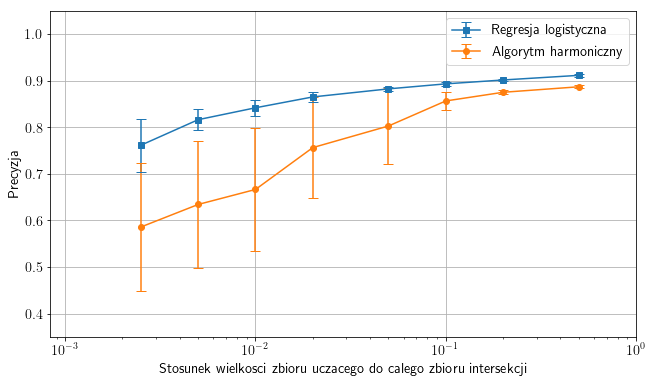
\includegraphics[width=0.95\linewidth]{img/results/wyniki-intersekcja.png}
	\caption{Wykres uzyskanej precyzji dla różnych rozmiarów zbioru uczącego, wykonane dla zbioru intersekcji.}\label{fig:wyniki-intersekcja}
\end{figure}